\chapter{Algoritmi e strategie di selezione degli elementi}

\section{Considerazioni iniziali e prerequisiti}

Al momento della registrazione delle azioni è indispensabile poter generare un selettore CSS che permetta di identificare in maniera univoca l'elemento interessato dall'interazione, per potervi accedere successivamente in fase di riproduzione. In aggiunta, il selettore individuato dovrebbe garantire una certa flessibilità ai cambiamenti che possono avvenire nel DOM durante lo sviluppo dell'applicazione, per non ritrovarsi con un insieme di test troppo fragili.
Allo stesso tempo però è necessario raggiungere un compromesso accettabile tra la resistenza alle variazioni e l'accuratezza delle verifiche, in modo che queste ultime permettano effettivamente di rivelare i problemi che si presentano.

La soluzione proposta parte da alcune considerazioni preliminari, basate principalmente sulla propria esperienza e sui criteri generali considerati come migliore prassi nella realizzazione di pagine web dinamiche, descritte di seguito. Tali punti non sono da considerarsi come vincoli necessari per il funzionamento dell'algoritmo, ma piuttosto come un'insieme di condizioni sotto le quali esso può esprime il suo funzionamento ottimale. 

\subsection {Validazione della sintassi HTML}

I risultati dell'algoritmo sono da considerarsi prevedibili solamente nel caso un cui il codice HTML della pagina web sia valido secondo la DTD dichiarata. Questa condizione presuppone che l'albero del DOM possa essere costruito in maniera corretta e che vengano eliminate possibili ambiguità, difficili da gestire in fase di analisi. I browser tentano di correggere gli errori di sintassi più comuni e spesso i problemi non sono così evidenti ad una semplice verifica visuale del contenuto mostrato. 

In particolare, l'algoritmo sfrutta in maniera intensiva la presenza e la distribuzione del l'attributo id per determinare quali elementi del DOM siano meno soggetti a potenziali cambiamenti. E' quindi importante che l'attributo id venga utilizzato in maniera corretta, secondo le specifiche del W3C, evitandone per esempio la duplicazione. Se per generare le pagine si utilizzano sistemi di gestione dei contenuti (CMS) spesso non si ha il controllo completo sul codice HTML prodotto, perciò in tali casi è bene assicurarsi che l'attributo venga adoperato in maniera adeguata.

Per ottenere i migliori risultati è quindi sempre consigliabile assicurarsi di validare il codice HTML delle pagine sotto esame attraverso uno strumento come il W3C Validator \footnote{\url{http://validator.w3.org}}. Le specifiche dettate da questo consorzio sono state utilizzate per stabilire un'insieme omogeneo di regole su cui fondare la strategia dell'algoritmo.

Se questo requisito non viene rispettato, potrebbe essere possibile perdere molti dei vantaggi forniti dall'algoritmo in termini di flessibilità ai cambiamenti strutturali delle pagine.

\subsection {Utilizzo dei tag HTML in maniera semantica}

Ogni tipologia di tag HTML disponibile è stato pensato per attribuire un certo significato semantico ai contenuti della pagina, e non solamente per regolarne l'aspetto con cui esso viene presentato. La scrittura di codice HTML semantico è oramai diventata una prassi consolidata nello sviluppo di applicazioni web moderne poiché i benefici ottenibili sono molteplici ed interessano ambiti diversi, dalla mantenibilità del codice all'indicizzazione sui motori di ricerca, passando per l'accessiblità.

L'algoritmo proposto cerca di sfruttare per quanto possibile il significato semantico attribuito ai vari elementi della pagina per reperire ulteriori informazioni e stabilire un selettore che tenga in considerazione le porzioni di pagina soggette a modifiche con maggiore probabilità.

Un uso attento della semantica implica generalmente anche la presenza di un minor numero di tag HTML nella pagina, ossia di un albero del DOM più compatto. Ciò favorisce evidentemente la robustezza dei test sull'interfaccia, sia perché riduce il numero di componenti che possono variare, sia perché i selettori generati sono più semplici ed effettivi. Per gli stessi motivi è opportuno affidare quanto più possibile ai fogli di stile la presentazione del contenuto, senza ricorrere ove non necessario all'aggiunta di codice di markup aggiuntivo per fini prettamente grafici.

In merito a questo criterio non possono esistere regole deterministiche e schemi prefissati da seguire. E' quindi responsabilità di chi si occupa dello sviluppo dell'interfaccia utente dell'applicazione web la scrittura di codice che faciliti la fase di verifica. L'algoritmo proposto cerca infatti di fornire supporto per stabilire la strategia di selezione degli elementi, ma l'uso di uno strumento automatico può sfruttare ma non può sostituire il lavoro svolto a monte per scrivere codice di qualità. Questa affermazione d'altronde è valida nell'ambito dei test in ogni dominio: più il codice sotto esame è ben organizzato, più sarà facile verificarne il funzionamento dall'esterno.

\section{Idee ed ipotesi di partenza}

Il funzionamento dell'algoritmo fonda le sue basi su di un modello empirico e non su concetti dimostrabili a priori, poiché le differenti casistiche che si presentano esaminando applicazioni web reali sono in numero potenzialmente infinito ed un'analisi rigorosa esula dagli obiettivi di questa trattazione. Pertanto i punti di partenza sono forniti dalla propria esperienza nella realizzazione di pagine e di applicazioni web utilizzando le tecnologie più recenti, e dall'osservazione diretta di casi significativi.

Gli spunti raccolti hanno contribuito a definire una serie di criteri adattabili alle situazioni comuni, attraverso i quali l'algoritmo tenta di risolvere i problemi tipici presenti nel test di applicazioni web. L'obiettivo principale è riuscire a stabilire un selettore CSS che identifichi l'elemento corretto nonostante le possibili modifiche che interessino i suoi attributi, quelli dei nodi appartenenti alla sua linea gerarchica e il suo posizionamento nel DOM. A seguire viene presentato un elenco delle variazioni più comuni, per chiarificare i concetti esposti fino ad ora.

\subsection {Schemi tipici di variazioni nel DOM}

Nella figura ~\ref{fig:domMod} sono presentati i principali schemi individuati secondo i quali avvengono le variazioni nel DOM durante il processo incrementale di sviluppo dell'applicazione web. Nei diagrammi sono evidenziati in arancione i nodi di interesse ai fini del test. 

Le modifiche rappresentate non pregiudicano in linea di massima il funzionamento della pagina in esame: si pensi ad esempio al caso comune in cui si aggiunga un tag div che funge da semplice contenitore, oppure all'aggiunta di una o più classi per ragioni stilistiche. E' quindi importante che il selettore tenga in considerazione queste potenziali variazioni in modo che l'elemento interessato sia reperibile anche seguito ad esse, pena il fallimento del test senza un effettivo difetto funzionale.

\begin{figure}[htbp]
\begin{center}
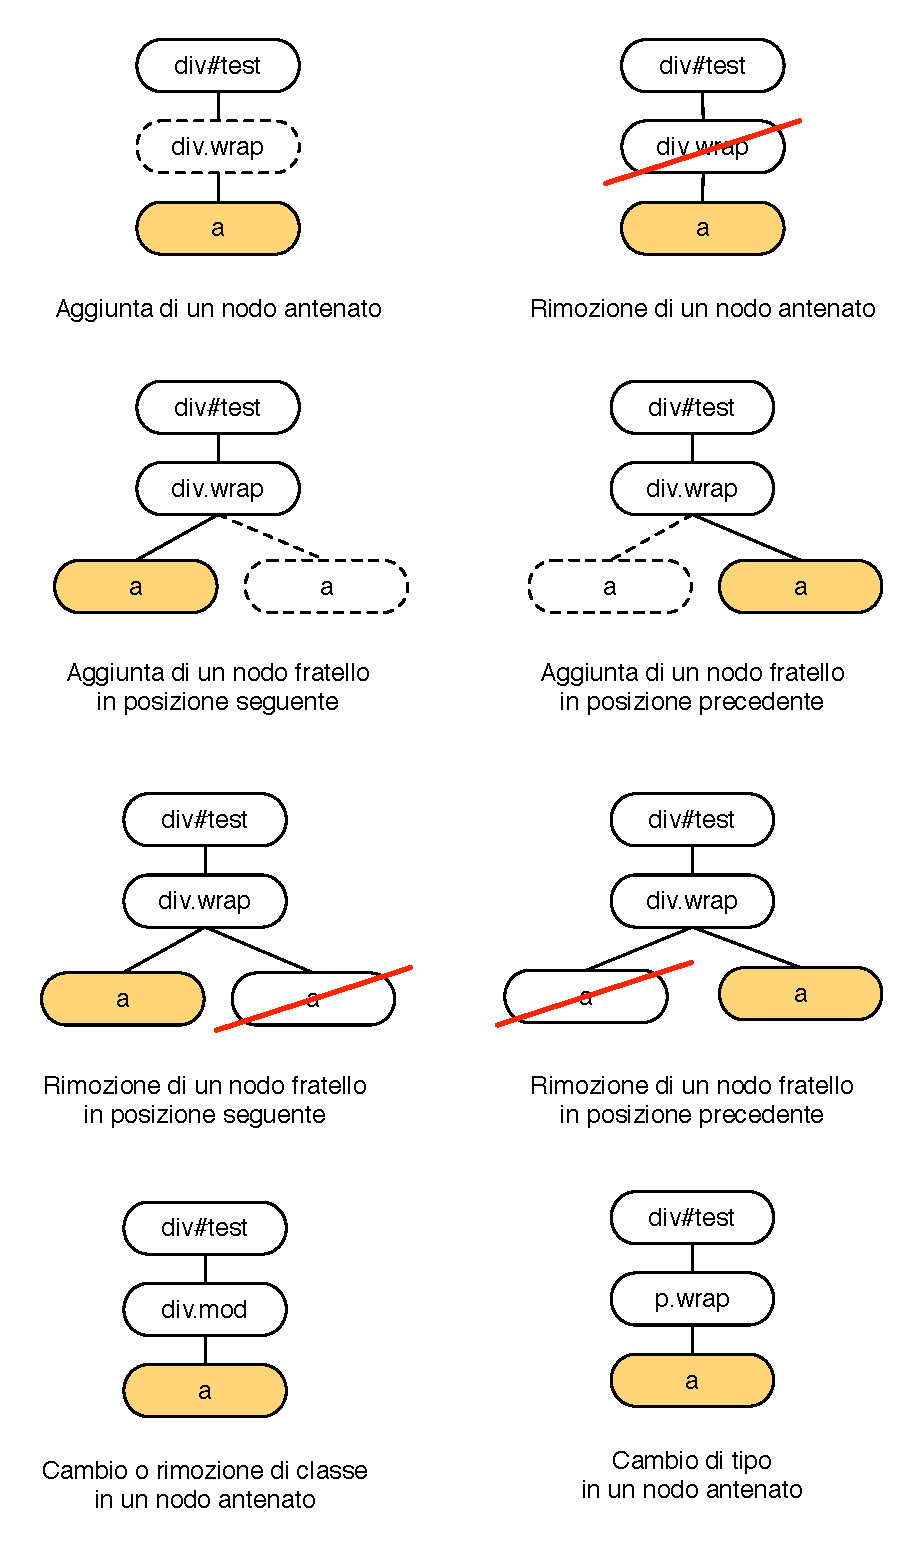
\includegraphics[width=0.7\textwidth]{images/dom_mod.eps}
\caption{Principali schemi di modifica del DOM}
\label{fig:domMod}
\end{center}
\end{figure}

\subsection {L'importanza dell'attributo id}

L'algoritmo proposto attribuisce una notevole importanza all'attributo id assegnabile ai tag HTML. Secondo la specifica W3C, l'attributo id deve essere utilizzato come identificatore univoco per un elemento della pagina \footnote{\url{http://www.w3.org/TR/html401/struct/global.html\#h-7.5.2}}. Di conseguenza, se in fase di scrittura dell'HTML si sceglie di assegnare questo attributo ad un tag, si può dedurre che esso agli occhi dello sviluppatore svolge un ruolo ben preciso ed ha pertanto la sua importanza nella pagina. Essendo univocamente identificato inoltre sarà sempre possibile accedere a tale elemento indipendentemente dal contesto in cui esso si trova. 

Inoltre, questo identificativo rappresenta il modo più performante e sicuro per accedere all'elemento da codice Javascript, tramite il metodo \verb|document.getElementById|. Siccome spesso l'id viene assegnato proprio con questo scopo, è relativamente poco probabile che esso venga modificato o rimosso in un secondo momento rispetto ad altri attributi, poiché ciò comporterebbe anche la potenziale modifica degli script sviluppati per l'applicazione.

Idealmente, se tutti gli elementi del DOM avessero un attributo id il problema che l'algoritmo tenta di risolvere sarebbe inesistente, poiché la selezione del nodo di interesse non dovrebbe tener conto della posizione nell'albero. Questa osservazione giustifica di fatto il peso che l'algoritmo gli assegna. 

Più l'albero del DOM è complesso, più alta è la probabilità che si verifichi prima o poi una variazione che interessi indirettamente il percorso verso il nodo di destinazione. L'algoritmo cerca pertanto di semplificare le condizioni di partenza lavorando su di un sottoalbero che contiene il nodo da selezionare. Come radice di tale sottoalbero viene scelto il primo nodo antenato che possiede un attributo id, incontrato visitando in maniera bottom-up la gerarchia. 

Nel caso banale in cui il nodo da selezionare possieda egli stesso un id, il sottoalbero conterrà un solo elemento. Negli altri casi invece si avrà come punto di partenza del selettore un nodo con attributo id, che quindi avrà le proprietà descritte poco prima, limitando quindi le potenziali combinazioni di variazioni relativamente alla struttura dell'intero documento. Per costruzione il selettore CSS risultante avrà in prima posizione un frammento di tipo id, che sarà anche l'unico presente, nel caso in cui nodo abbia almeno un elemento antenato con questo attributo impostato. 

\begin{figure}[htbp]
\begin{center}
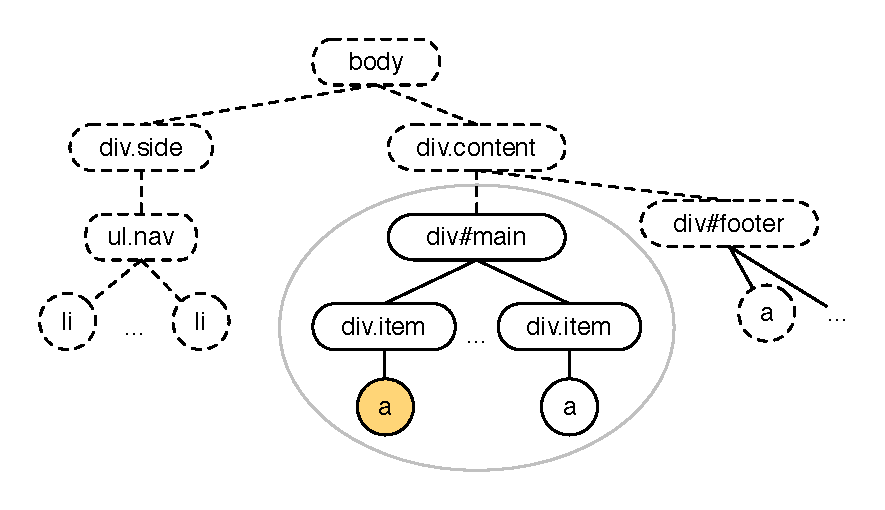
\includegraphics{images/id_partition.eps}
\caption{Identificazione del sottoalbero a partire dall'ID}
\label{fig:idPartition}
\end{center}
\end{figure}

Il problema di selezionare in modo flessibile i vari componenti in fase di testing è una problematica che come si è detto interessa anche le applicazioni tradizionali con interfaccia grafica. In questo ambito una delle soluzioni spesso utilizzate comporta l'utilizzo di una o più classi ausiliarie che svolgono il ruolo di repository per i componenti. Tramite queste classi è possibile accedere in maniera opaca ai vari widget durante i test, poiché esse implementano al loro interno la logica per individuare il componente, mappandone la reale posizione ad un identificativo. Quando viene modificata la struttura dell'interfaccia, è quindi sufficiente modificare il codice in un solo punto, senza modificare l'implementazione dei test.

Nel caso delle applicazioni web con interfaccia in HTML, l'attributo id può svolgere concettualmente lo stesso ruolo dell'identificativo nel repository dei widget, con il vantaggio che questa possibilità è intrinseca alla tecnologia utilizzata.

Durante lo sviluppo dell'interfaccia è buona norma quindi procedere con un occhio di riguardo per la successiva fase di acceptance testing e adoperare gli accorgimenti necessari per renderla più agevole. Per quanto visto fino ad ora, può essere molto utile assegnare gli attributi id agli elementi più importanti della pagina, che permettono all'utente di attivare le funzionalità principali oppure che forniscono le informazioni di maggiore interesse, e tenere il più possibile costanti i valori di questi identificativi durante le successive modifiche, in modo da non influenzare i test definiti.

\subsection {L'attributo role}

Un altro importante attributo utilizzato dall'algoritmo è l'attributo \verb|role|. Se presente, esso serve ad indicare uno o più ruoli che l'elemento possiede nell'ambito della pagina. Un corretto uso semantico di questo attributo viene illustrato nella specifica del W3C \footnote{\url{http://www.w3.org/TR/xhtml-role/\#s_role_module_attributes}}:

\lstinputlisting[float=h, language=Html, caption={Esempio di uso semantico dell'attributo role}, label=code:roleAttr]{code/selector/w3c_role.html}

Se chi ha scritto il codice HTML ha definito questo attributo per un tag in particolare, con molta probabilità il suo valore può essere un buon candidato per selezionare l'elemento stesso in mancanza di un attributo id, oppure per costruire il percorso verso l'elemento da selezionare se l'attributo si trova su di un elemento antenato. 

In quest'ultimo caso l'attributo \verb|role| può aiutare ad identificare il sottoalbero in cui si trova l'elemento di interesse, corrispondente ad un'area nella pagina web.

\subsection {Selettori per elementi particolari}

In base al tipo e valore semantico dell'elemento da selezionare, l'algoritmo stabilisce una strategia apposita per un sottoinsieme di elementi DOM che hanno attributi di particolare significato:

\begin{description}
\item[Campi di input] Alcuni tipi di tag HTML sono definiti per permettere all'utente di inserire dei dati in ingresso, processabili poi lato server. La loro strategia di selezione è pertanto fondamentale in fase di testing. Per questi elementi di input, come caselle di testo, caselle di spunta, menù a tendina, è di particolare interesse l'attributo \verb|name|. 

Il valore assegnato a tale attributo viene utilizzato nell'invio della richiesta HTTP successiva alla sottomissione del form come chiave che identifica il dato inserito dall'utente nel relativo campo. Lato server l'applicazione utilizza quindi il valore dell'attributo \verb|name| per accedere al dato inviato. Siccome esiste questa dipendenza, è meno probabile che l'attributo name venga modificato in seguito a modifiche grafiche nel layout della pagina.Per questo motivo, esso è un ottimo candidato per identificare in maniera consistente e robusta il nodo del DOM in mancanza dell'attributo id.

\item[Label] Il tag \verb|label| è stato definito per comunicare all'utente il tipo di dato da inserire in un campo di testo. L'algoritmo ne utilizza l'alttributo \verb|for|, che se presente specifica l'id del campo di input a cui si riferisce il testo dell'etichetta. Per gli stessi motivi indicati nel punto precedente è possibile sfruttare questa informazione aggiuntiva nel selettore generato.

\item[Liste] Per definire liste ordinate di elementi in una pagina in maniera semantica si utilizza l'apposito tag \verb|ol|. Nel selettore CSS che individua una voce specifica della lista, l'algoritmo specifica sempre l'ordine, utilizzando lo pseudo selettore \verb|:eq(n)| messo a disposizione dalla libreria jQuery, che estende le capacità dei selettori CSS con alcune caratteristiche aggiuntive.

\item[Collegamenti ipertestuali] Anche i collegamenti ipertestuali giocano un ruolo centrale durante la fase di testing. Nel caso in cui non siano definiti attributi di tipo id o class, l'algoritmo utilizza lo pseudo selettore \verb|:contains()| di jQuery, che seleziona un elemento in base al testo contenuto.

Le alternative analizzate per questo particolare caso sono state la selezione in base alla posizione rispetto al nodo padre oppure in base all'url specificato nell'attributo \verb|href|. Entrambe però si sono però rivelate meno efficaci. La posizione è infatti una variabile poco significativa, che rende la selezione troppo fragile alle modifiche. Il valore dell'alttributo \verb|href| invece è stato scartato poiché l'url di un link è frequentemente soggetto a modifiche interne all'applicazione, anche di piccola entità, come l'aggiunta di un parametro alla querystring.

\end{description}

\subsection {Descrizione dell'algoritmo}

All'interno dell'applicazione sviluppata, si è implementato l'algoritmo proposto utilizzando il linguaggio Javascript e la libreria jQuery. Quest'ultima è stata impiegata in questo ambito per due motivi. 

In primo luogo, jQuery fornisce dei metodi di navigazione dell'albero DOM molto potenti e di comodo utilizzo, senza bisogno di dover ricorrere all'API di Javascript per reimplementare queste funzionalità. 

In secondo luogo, jQuery estende le capacità dei selettori CSS3 con nuovi pseudo-selettori, che in alcuni casi rappresentano una scorciatoia per selettori più complessi usati frequentemente, mentre in altri casi esprimono criteri di selezione non definibili tramite i selettori standard. In aggiunta, è possibile ampliare questo insieme di pseudo-selettori realizzandone di personalizzati se necessario.

Il funzionamento dell'algoritmo per la generazione dei selettori CSS è diviso in due fasi distinte. 

Nella prima fase si costruisce in maniera ricorsiva il selettore, partendo dal nodo di interesse e visitando l'albero in maniera bottom-up. Durante questo processo sono tenuti in considerazione i criteri esposti in precedenza per comporre le singole parti del selettore, basandosi sull'elemento corrente in ogni iterazione.

Nella seconda fase il selettore così ottenuto viene ottimizzato dal punto di vista delle potenziali variazioni future subite dall'albero del DOM. Procedendo per tentativi l'algoritmo elimina le componenti superflue dal selettore, per ottenerne uno minimo.

L due fasi vengono descritte nel dettaglio nei paragrafi seguenti.

\subsubsection {Prima fase: percorso bottom-up}

La prima fase viene realizzata attraverso la funzione \verb|_traverse|. Come parametro in ingresso l'algoritmo si aspetta un riferimento ad un oggetto Javascript che rappresenta il nodo del DOM da selezionare. I passaggi dell'algoritmo sono i seguenti:

\begin{enumerate}
\item Se l'elemento corrente è il tag \verb|body|, la ricorsione termina e si restituisce il selettore generato finora, poiché si è raggiunta la radice dell'albero.
\item Viene prodotto il frammento del selettore che identifica l'elemento corrente:
	\begin{enumerate}
		\item Se per l'elemento corrente è stato definito l'attributo id, questo viene aggiunto  in fronte al selettore costruito fino ad ora.
		\item Se l'elemento è di tipo \verb|a|, viene preposto il frammento \verb|a:icontains()|, che seleziona il nodo contenente il testo specificato nelle parentesi dello pseudo-selettore jQuery.
		\item Se l'elemento possiede uno o più attributi \verb|role|, viene aggiunto un frammento del tipo \verb|<tipotag>[role=<role>]|.
		\item Se l'elemento è un widget di input e possiede l'attributo \verb|name|, si aggiunge un frammento del tipo \verb|<tipotag>[name=<name>]|
		\item Se l'elemento è una label è presente l'attributo \verb|for| e nella pagina esiste un nodo con attributo id uguale al valore dell'attributo for, si aggiunge un frammento del tipo \verb|<tipotag>[for=<for>]| 
		\item Se l'elemento è una voce di un elenco numerato, viene specificato il numero ordinale che ne indica la posizione tra i figli del nodo \verb|ol| genitore, tramite lo pseudo-selettore \verb|:eq(<indice>)|
		\item Se l'elemento possiede una o più classi, viene presa la prima in ordine di definizione e aggiunto in cima allo stack un componente al selettore del tipo \verb|.<classe>|
		\item Infine, se nessuna delle condizioni precedenti è applicabile, si aggiunge al selettore il nome del tag corrente.
	\end{enumerate}
\item Si verifica se il selettore costruito fino a questo punto identifica uno ed un solo elemento tra tutti i figli del genitore del nodo corrente:
	\begin{enumerate}
		\item Se la verifica ha esito positivo, il selettore generato fino a questo punto è univoco. Si continua la ricorsione invocando il metodo \verb|_traverse| con argomenti il padre dell'elemento attuale, che diventerà l'elemento corrente della prossima iterazione, e il vettore contenente le componenti del selettore.
		\item In caso contrario, esistono almeno due nodi nella partizione dell'albero visitata che rispondono allo stesso selettore. Siccome questo sarà sempre vero anche per le iterazioni successive, è necessario rimediare subito al problema. Per far ciò, si ricava l'indice posizionale dell'elemento identificato dal selettore in cima allo stack dei frammenti, relativamente al nodo genitore. Si appende poi a tale frammento lo pseudo-selettore \verb|:eq(<indice>)|. Poiché questa operazione viene effettuata ad ogni iterazione dell'algoritmo, si ha la certezza che il selettore così ottenuto sia univoco per costruzione, poiché l'indice posizionale è sicuramente discriminante in caso di ambiguità.
	\end{enumerate}	
	
\end{enumerate}

Al termine di questo procedimento si ottiene quindi un selettore univoco per l'elemento iniziale, composto da un frammento per ogni livello del DOM incontrato nella visita.

\subsubsection {Seconda fase: ottimizzazione del selettore}

Il selettore ottenuto tramite la fase precedente viene semplificato per ottenere un nuovo selettore che identifichi lo stesso elemento di partenza, ma che sia più resistente alle potenziali modifiche apportate alla struttura della pagina.

La fase di ottimizzazione si basa sulla seguente ipotesi, basata sull'osservazione del punto dell'albero DOM in cui avvengono le modifiche durante lo sviluppo dell'interfaccia nel lungo periodo. Considerando come punto di riferimento la posizione nel DOM del nodo selezionato per il test, è più probabile che le modifiche si verifichino nei livelli gerarchici più vicini al punto di riferimento, piuttosto che nei livelli più distanti. Si identifica quindi una certa località nella distribuzione delle modifiche rispetto al nodo di interesse.

Questa ipotesi si fonda sul fatto che la struttura di una pagina web segue normalmente uno schema comune, nella quale gli elementi più in alto nel DOM sono utilizzati per definire la struttura di base del layout grafico, come l'intestazione della pagina, l'area dei contenuti principali, la barra di navigazione laterale. E' ragionevole supporre che, una volta definite, queste macroaree rimarranno stabili e non subiranno modifiche continue durante lo sviluppo incrementale dell'interfaccia.

Viceversa, saranno gli elementi più interni a subire il maggior numero di modifiche, con l'aggiunta di nuovo contenuto, nuove voci nei menù, e la riorganizzazione delle strutture interne.

Basandosi su tali considerazioni, l'algoritmo prova a rimuovere progressivamente i frammenti del selettore, partendo dal frammento subito precedente a quello riferito al nodo di interesse, che rimane pertanto sempre presente. Se il selettore ottenuto continua ad identificare univocamente lo stesso elemento di partenza, il frammento corrente viene rimosso e si continua con quello che lo precede. Il procedimento viene interrotto quando si raggiunge il primo frammento di tipo id.

Di seguito vengono esposti nel dettaglio i vari passaggi di questa fase:

\begin{enumerate}
\item Si marca il nodo di partenza aggiungendovi una classe speciale, per verificare successivamente se il selettore ottimizzato continua ad identificare lo stesso elemento.
\item Il vettore \verb|path| è popolato con i frammenti del selettore ottenuto dalla fase precedente. In prima posizione è presente il frammento più generico, in ultima quello relativo al nodo di partenza.   
\item Per ogni elemento del vettore \verb|path|, partendo dal penultimo e procedendo con indice decrescente:
	\begin{enumerate}
		\item Se il frammento corrente è di tipo id, si interrompe l'iterazione e si ritorna il selettore corrente
		\item In caso contrario, si duplica il vettore, si rimuove dalla copia il frammento corrente e si compone il nuovo selettore unendo gli elementi del vettore di prova.
		\item Si recupera l'insieme dei nodi del DOM che rispondono a tale selettore di prova e si verifica che esso sia composto da un unico elemento. Inoltre, questo elemento deve possedere la classe speciale usata come marcatore, per assicurarsi che il selettore identifichi esattamente il nodo di partenza.
		\item Se queste condizioni sono verificate, il vettore di prova diventa il vettore del selettore corrente. L'algoritmo procede e l'analisi si sposta sul frammento in posizione precedente.
	\end{enumerate}
\end{enumerate}

\subsection {Esempi pratici di funzionamento}

Verranno ora presentati alcuni esempi pratici di funzionamento dell'algoritmo in scenari d'uso interessanti ai fini della trattazione. Per ogni esempio saranno indicati il selettore ottenuto dalla prima fase, quello finale dopo l'ottimizzazione, e le peculiarità del caso in esame.

Nelle figure inserite si sono evidenziati in rosso il nodo di interesse, preso come punto di partenza dall'algoritmo, in giallo i noti aggiunti o modificati dopo un'ipotetica modifica alla pagina web.

\subsubsection {Aggiunta di elementi contenitori multipli}

Selettore non ottimizzato:  \verb|#content .foo div p| 
\newline
Selettore finale:  \verb|#content p| 

\begin{figure}[htbp]
\begin{center}
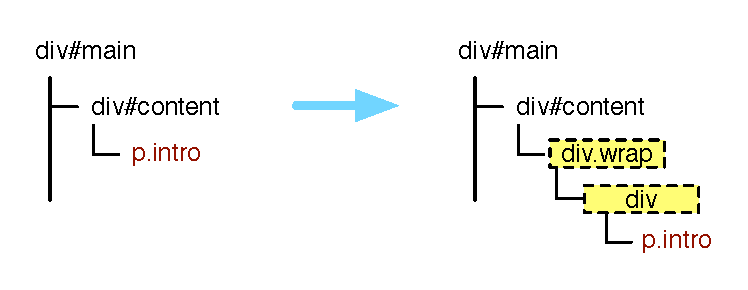
\includegraphics[width=\textwidth]{images/dom_examples/wrap.eps}
\end{center}
\end{figure}

Il selettore ottimizzato non contiene riferimenti ai nodi intermedi e pertanto continua a selezionare l'elemento corretto anche dopo la modifica evidenziata. Grazie al partizionamento dell'albero basato sull'attributo id più vicino, il selettore si comporterebbe in maniera corretta anche se venisse aggiunto un paragrafo con classe \verb|intro| direttamente sotto il div con id \verb|main|

\subsubsection {Aggiunta di una nuova voce in un menù a più livelli}

Selettore non ottimizzato:  \verb|#menu > li:eq(1) ul > li:eq(1) a:icontains(item3)| 
\newline
Selettore finale:  \verb|#menu a:icontains(item3)| 

\begin{figure}[htbp]
\begin{center}
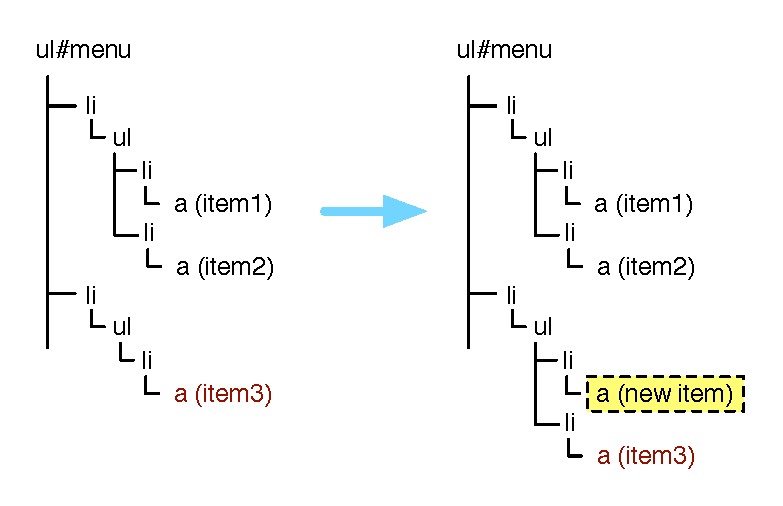
\includegraphics[width=\textwidth]{images/dom_examples/menu_add_item.eps}
\end{center}
\end{figure}

Questo scenario rappresenta un caso tipico di modifica apportata al menù di un'applicazione web, ossia l'aggiunta di una voce di menù. L'elemento di interesse è il collegamento ipertestuale con testo "item3" e prima di esso viene aggiunta la nuova voce. 

Come si può notare, il selettore non ottimizzato contiene riferimenti espliciti alla posizione delle voci della lista non ordinata, poiché nessuno dei tag \verb|li| o \verb|a| possiede un attributo di classe. L'unico modo per ottenere un selettore non ambiguo consiste nello specificare l'indice tramite lo pseudo selettore \verb|:eq()|. Inoltre, il nodo finale di tipo \verb|anchor| viene identificato tramite il testo in esso contenuto, tramite lo pseudo selettore \verb|:icontains()|. Per i collegamenti ipertestuali, nella maggior parte dei casi in cui mancano altri attributi più specifici, il testo contenuto nel nodo si rivela un buon elemento di discriminazione, migliore della posizione.

Se l'algoritmo non effettuasse l'ottimizzazione, il selettore risultante non sarebbe sufficientemente flessibile da selezionare comunque la stessa voce del menù in seguito all'aggiunta di una nuova voce in posizione antecedente ad essa, poiché l'indice posizionale risulterebbe alterato.

Durante l'ottimizzazione vengono rimossi questi vincoli di posizione, che di fatto risultano essere ridondanti, poiché esiste un solo tag di tipo \verb|a| che contiene il testo specificato all'interno del sottoalbero che ha \verb|ul#menu| come radice. Grazie a questo accorgimento, il selettore continua  a funzionare anche dopo le modifiche, rendendo i test che lo utilizzano meno fragili. Il risultato che si ottiene è del tutto analogo qualora lo scenario prevedesse la rimozione di una voce di menù invece che l'aggiunta.

\subsubsection {Utilizzo semantico di una lista ordinata}

Selettore non ottimizzato:  \verb|#ordered li:eq(0) a:icontains(item 1)| 
\newline
Selettore finale:  \verb|#ordered li:eq(0) a:icontains(item 1)| 

\begin{figure}[htbp]
\begin{center}
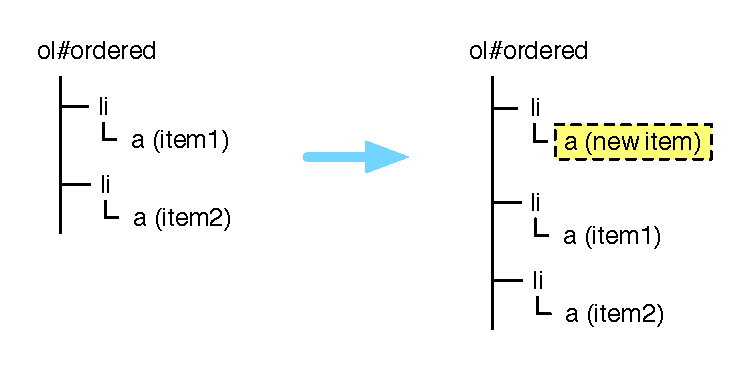
\includegraphics[width=\textwidth]{images/dom_examples/ordered_menu.eps}
\end{center}
\end{figure}

A differenza dello scenario precedente, questa volta viene utilizzata una lista ordinata. L'algoritmo utilizza questa informazione semantica e forza nel selettore ottimizzato la presenza dell'indice posizionale. Pertanto il selettore non sarà in grado di identificare alcun elemento dopo le modifiche evidenziate. Siccome si è specificato un tag \verb|ol|, chi ha sviluppato l'interfaccia grafica ha voluto sottolineare l'importanza dell'ordine nell'elenco. L'algoritmo raccoglie questa indicazione semantica e se il selettore viene utilizzato in un test, esso fallirà in seguito all'aggiunta di una nuova voce antecedente poiché non sarà possibile reperire l'elemento specificato.

La verifica dell'ordine può essere infatti un requisito fondamentale nel caso in cui ci si voglia accertare che un menù compaia esattamente come richiesto dal committente, oppure per questioni di accessibilità o comodità d'uso.

\subsubsection {Campi di input}

Selettore non ottimizzato:  \verb|#test > .input:eq(0) input[name=title]| 
\newline
Selettore finale:  \verb|#test input[name=title]| 

\begin{figure}[htbp]
\begin{center}
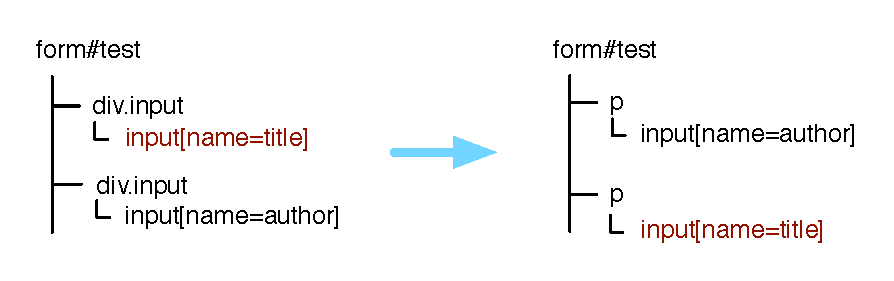
\includegraphics[width=\textwidth]{images/dom_examples/form1.eps}
\end{center}
\end{figure}

Per selezionare un campo di input viene utilizzato preferibilmente il valore dell'attributo \verb|name|. Nel caso mostrato in figura, il selettore generato è abbastanza flessibile da continuare a funzionare anche dopo il cambiamento di tipo e di ordine degli elementi contenitori.

Se invece venisse modificato l'attributo \verb|name| il selettore non sarebbe in grado di accedere al campo di input e sarebbe necessario modificare il test, in modo che rifletta le modifiche apportate. Questa situazione è comunque ragionevole poiché il cambio di nome presuppone un potenziale cambiamento anche alla parte dell'applicazione lato server, pertanto è opportuno ridefinire il passaggio del test interessato per non rischiare di ottenere un falso risultato positivo.

\subsection {Unit test dell'algoritmo}

Il funzionamento dell'algoritmo proposto è stato verificato attraverso un insieme di unit test definiti in Javascript tramite QUnit, un framework di testing realizzato dal team di jQuery \footnote{\url{http://docs.jquery.com/QUnit}}. 

Gli unit test verificano l'unicità dell'elemento individuato e la corrispondenza con l'elemento di partenza. Inoltre, gli scenari proposti in precedenza costituiscono il corpo di alcuni dei test effettuati per misurare la flessibilità dei selettori generati rispetto alle modifiche nel DOM.

\section{Algoritmo di generazione dei selettori alternativi}

Durante la fase di riproduzione dei test, i selettori generati dall'algoritmo vengono utilizzati per identificare gli elementi della pagina su cui simulare gli eventi o effettuare le verifiche specificate dalle asserzioni.

Nell'ottica di migliorare ulteriormente la resistenza dei test alle modifiche, è stato implementato un secondo algoritmo. Esso può essere utilizzato durante la fase di riproduzione per effettuare alcuni tentativi aggiuntivi nel caso in cui non sia possibile individuare nella pagina un nodo del DOM che risponda al selettore specificato nel test.

Questo secondo algoritmo stabilisce quindi alcuni criteri per ottenere un insieme di selettori alternativi a quello di partenza attraverso i quali lo strumento di test tenta di reperire l'elemento di interesse. 

Si noti che è comunque necessario sottostare ad un compromesso tra la resistenza del test alle modifiche e l'accuratezza delle verifiche effettuate. Se si favorisce eccessivamente il primo tra questi due aspetti, ci si potrebbe trovare con una serie di test che non sono sensibili a potenziali malfunzionamenti dell'applicazione.

Pertanto si è scelto di applicare questo algoritmo soltanto per alcuni tipi di operazioni durante la riproduzione dei test, per le quali risulta poco probabile che il maggior grado di flessibilità fornito possa creare dei falsi positivi nei risultati. Tra tutte le operazioni definibili in un test, quelle rivelatesi più adatte per l'applicazione dell'algoritmo sono state le azioni che simulano la navigazione dell'utente tra le pagine, come il click su di un link o su di un bottone per l'invio di un form.

Durante la riproduzione di queste operazioni infatti è possibile avvantaggiarsi di un margine di tolleranza più ampio nell'accuratezza con cui si identifica dell'elemento obiettivo nella pagina, poiché il rischio di fornire un falso positivo come risultato del test è minore. Per avvalorare questa ipotesi con un esempio pratico, si può osservare che se venisse simulato il click su di un link differente da quello specificato nei test, fallirebbero comunque con grande probabilità tutti i test successivi, definiti su di una pagina che non è in realtà quella caricata dopo il click sul link errato.

Viceversa per altri tipi di operazioni, come le asserzioni riguardo il contenuto di alcune porzioni della pagina, è preferibile utilizzare il selettore CSS per l'elemento da verificare esattamente come è stato specificato nel test, poiché i selettori alternativi proposti dall'algoritmo potrebbero portare a risultati ambigui.

\subsection{Principi di base e funzionamento}

Per proporre i selettori alternativi a quello di partenza, durante ogni iterazione dell'algoritmo vengono eliminati i frammenti ai quali viene assegnato un peso minore, in modo da ottenere un selettore via via meno specifico. 

Anche in questo caso, i selettori alternativi vengono proposti in base a due principi già sfruttati per l'algoritmo di generazione del selettore. Il principio di località delle modifiche descritto in precedenza in questo caso viene applicato non direttamente al DOM ma alla gerarchia identificata dal selettore. Ad ogni frammento viene assegnato un certo peso durante la fase di preparazione iniziale, successivamente valutato per decidere l'ordine in cui rimuovere i frammenti. I frammenti considerati meno indicativi saranno rimossi nei primi selettori alternativi proposti. L'unico frammento che non verrà rimosso sarà quello in ultima posizione nel selettore di partenza, poiché si riferisce direttamente all'elemento da ricercare. 

Una volta assegnato il peso a ciascun frammento, essi saranno eliminati secondo l'ordinamento rispetto del peso assegnato. Quindi, la probabilità che un frammento venga eliminato durante le prime iterazioni cresce in base al peso assegnatogli.

Nel calcolo del peso di ogni frammento vengono conteggiati due fattori. La prima componente è fissa ed è assegnata in base al tipo di frammento. Il contributo minimo viene assegnato ai frammenti di tipo \verb|id|, per le stesse motivazioni già esposte in precedenza. Il valore assegnato cresce poi per i frammenti di tipo \verb|.class|, fino ad ottenere il valore minimo per i frammenti che specificano solamente il tipo di tag.

La seconda componente invece è proporzionale alla posizione che il frammento occupa nel selettore iniziale. Più sarà distante dal frammento che specifica l'elemento interessato, più il contributo sarà maggiore. Pertanto, a parità di tipo, i frammenti nelle posizioni iniziali avranno un peso maggiore, mentre quelli nelle posizioni finali avranno un peso minore. Questa strategia di fatto sfrutta l'idea della località delle modifiche, poiché i frammenti relativi ad elementi del DOM più vicini a quello selezionato in partenza saranno eliminati per primi con maggiore probabilità nei tentativi effettuati.

Di seguito viene proposta la sequenza delle operazioni compiute dall'algoritmo

\begin{enumerate}
\item La stringa del selettore di partenza viene spezzata e i frammenti inseriti in un vettore
\item Se il vettore contiene un solo elemento, l'algoritmo restituisce l'elemento specificato dal selettore originale, poiché ci si trova in un caso banale e non è possibile proporre alternative.
\item Ogni elemento del vettore viene passato alla funzione \verb|buildItem|, che crea la struttura dati necessaria ed assegna il peso al frammento;
	\begin{enumerate}
		\item Se il frammento corrente è di tipo id, viene assegnato il peso minimo, pari ad 1.
		\item Se il frammento è del tipo \verb|tag.classe|, viene assegnato un peso pari a 10.
		\item Se il frammento specifica solamente una classe, viene assegnato un peso pari a 50.
		\item Se il frammento indica unicamente il tipo del tag, viene assegnato un peso pari a 100.
		\item Il peso assegnato viene moltiplicato per la posizione che il frammento occupa nel vettore.
	\end{enumerate}
\item Finché il vettore dei frammenti contiene almeno un elemento:
	\begin{enumerate}
		\item Si verifica se il selettore costruito dal vettore dei frammenti corrente selezioni un elemento del DOM.
		\item Se ciò è vero, l'algoritmo termina e viene restituito un riferimento al nodo individuato dal selettore corrente.
		\item In caso contrario, si rimuove dal vettore corrente il frammento a cui è assegnato il peso maggiore tra quelli presenti e si procede con l'iterazione successiva.
	\end{enumerate}	
\item Se si è raggiunto il numero massimo di tentativi consentiti senza riuscire ad individuare alcun elemento, viene restituito un riferimento nullo.
\end{enumerate}

Se è necessario, è possibile adattare il comportamento dell'algoritmo all'applicazione in esame agendo in due punti: modificando il criterio di assegnazione dei pesi si modifica l'ordine dei tentativi effettuati, privilegiando un tipo di frammento piuttosto che un altro; regolando il numero di tentativi effettuati si aumenta o diminuisce il grado di sensibilità alle variazioni nella struttura della pagina.